
\documentclass[11pt]{article}

\usepackage[margin=1in]{geometry}
\usepackage[T1]{fontenc}
\usepackage[utf8]{inputenc}
\usepackage{lmodern}
\usepackage{enumitem}
\usepackage{amsmath}
\usepackage{amssymb}
\usepackage{graphicx}
\usepackage{booktabs}
\usepackage{hyperref}

\setlength{\parindent}{0pt}
\setlength{\parskip}{0.4em}
\setlist[itemize]{leftmargin=1.2em, topsep=0.2em, itemsep=0.15em}
\setlist[enumerate]{leftmargin=1.4em, topsep=0.2em, itemsep=0.15em}

\begin{document}

\begin{center}
{\Large \textbf{Milestone 2 Design Report}}\\[0.4em]
{\large GPU-Accelerated TEBD for the 1D Transverse-Field Ising Model}
\end{center}

\textbf{Team members:} Xin Wei, Chiling Han, Hercy Shen\\
\textbf{Course:} CME 213: Parallel Computing with CUDA, MPI and OpenMP

\vspace{0.5em}

\textbf{1. Project Scope}

We are building a GPU TEBD solver for real-time dynamics of the 1D transverse-field Ising model
\[
H = -J \sum_i \sigma^x_i \sigma^x_{i+1} \;-\; g \sum_i \sigma^z_i,
\]
evolved from a product state on a Matrix Product State (MPS).

The user gives us $L$, $(J, g)$, an initial product state, $dt$, $t_{\max}$, maximum bond dimension $\chi_{\max}$, and Trotter order. We return the time series of magnetisations $\langle\sigma^z_i\rangle$, $\langle\sigma^x_i\rangle$, two-point correlations, bipartite entanglement entropy on every cut, the bond-dimension profile, and the accumulated SVD truncation error.

We assume open boundaries, $d = 2$, nearest-neighbour bonds, and a hand-written one-sided Jacobi SVD (no LAPACK). The project is a success if the CUDA TEBD reproduces our CPU reference against exact diagonalisation to machine precision and shows a clear speed-up on \texttt{update\_bond} once $\chi \gtrsim 32$. A multi-GPU mode for parameter sweeps via MPI is the M4 stretch goal.

\textbf{Status at M2.} The CPU reference is complete. All 54 unit tests pass. Against ED on $L = 8$, $dt = 0.05$, order 4, the final fidelity drop is $4.3 \times 10^{-11}$ (Sec.~6).

\vspace{0.4em}
\textbf{2. Related Work}

The MPS / TEBD foundations are Vidal's original paper and Schollw\"ock's review. Mature CPU/Python implementations include TeNPy, ITensor, quimb, and TensorNetwork. Our CPU reference uses the right-canonical Vidal-B form and the gate-cache structure from TeNPy.

GPU TEBD is less standardised. NVIDIA's cuTensorNet provides batched contractions and SVD on a single GPU, and ITensor supports MPI for independent runs. We are not advancing the state of the art: the goal is a clean, instrumented TEBD where every kernel is visible, so we can attribute time to gate contraction, SVD, and memory traffic without hiding behind a library. Our parallel one-sided Jacobi SVD follows the Brent--Luk pattern; the Trotter splitting follows Hatano--Suzuki.

\vspace{0.4em}
\textbf{3. Computational Challenges}

\begin{itemize}
    \item \textbf{SVD is the bottleneck.} Each TEBD sub-step performs $L-1$ complex SVDs of size up to $2\chi \times 2\chi$. We use one-sided Jacobi: non-overlapping column pairs are independent within a sweep, which maps cleanly to thread blocks. Convergence is data-dependent (5--10 sweeps in practice), so load balancing across bonds is non-trivial.

    \item \textbf{Tensor transposes are memory-bound.} \texttt{update\_bond} permutes $(2\chi)^2 \cdot d^2$ complex doubles per bond inside \texttt{tensor\_contract}. The permutation order matters for coalescing on the GPU.

    \item \textbf{Bond dimension saturates the budget.} Our quench data (Fig.~1) show the actual $\chi(t)$ rising to $\chi_{\max} = 64$ at $t \approx 1.9$ and the truncation error crossing $10^{-6}$ near $t \approx 3.85$. Cost per bond scales as $\mathcal{O}(\chi^3)$, so doubling the \emph{effective} bond dimension is an $8\times$ hit. Pre-allocating to $\chi_{\max} \cdot d \cdot \chi_{\max}$ (already done) avoids \texttt{cudaMalloc} during evolution.

    \item \textbf{Single-chain parallelism is limited.} Even and odd bonds within a sub-step are independent --- $(L-1)/2$-way parallelism, useful on a single GPU but limiting for strong-scaling across multiple GPUs on one chain.
\end{itemize}

\begin{figure}[h]
\centering
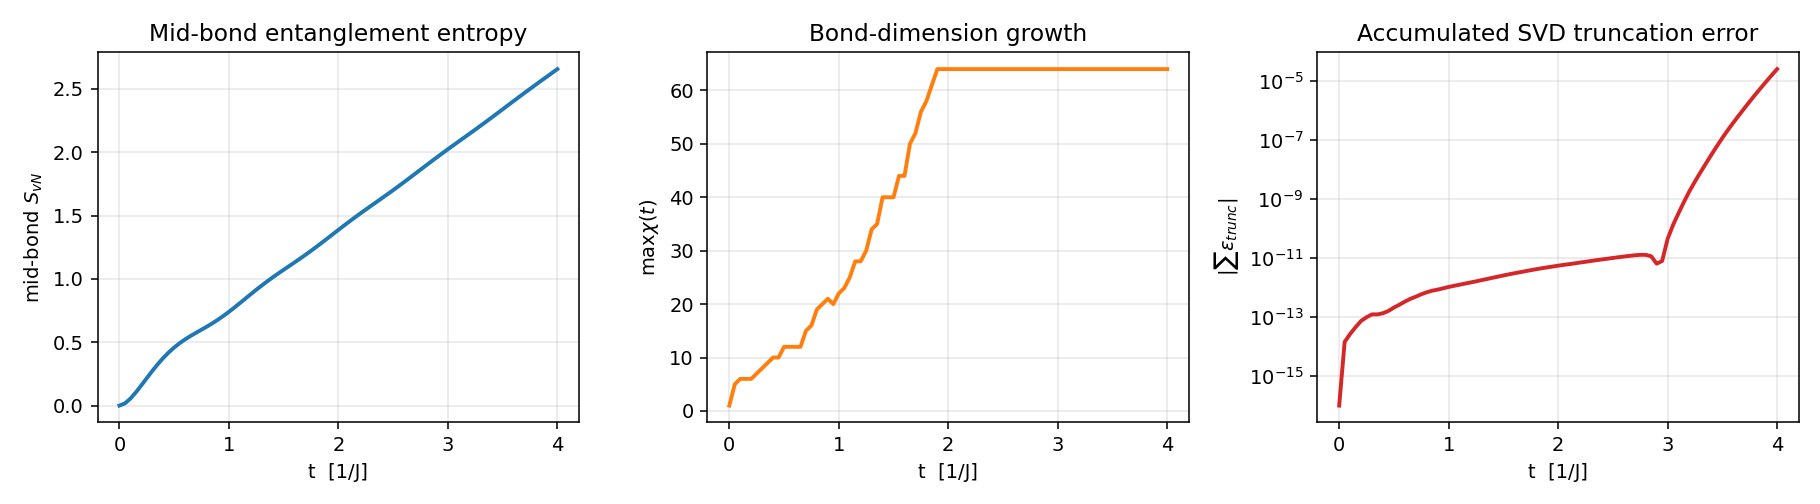
\includegraphics[width=\textwidth]{figs/summary.png}
\caption{$L = 20$ quench under TFIM ($J = g = 1$, $dt = 0.05$, order 4, $\chi_{\max} = 64$). Mid-bond entropy grows linearly; bond dimension saturates at $\chi_{\max}$ around $t \approx 1.9$; truncation error crosses $10^{-6}$ near $t \approx 3.85$.}
\end{figure}

\vspace{0.4em}
\textbf{4. CUDA Implementation Plan}

The CPU reference was built module-by-module to be CUDA-portable.

\begin{center}
\begin{tabular}{ll}
\toprule
\textbf{CPU routine} & \textbf{GPU implementation} \\
\midrule
\texttt{zgemm}            & tiled shared-memory kernel; \texttt{cublasZgemm} reference \\
\texttt{tensor\_contract} & transpose kernel + \texttt{zgemm} \\
\texttt{svd} (Jacobi)     & one block per non-overlapping column pair; sweep loop on host \\
\texttt{update\_bond}     & fused kernel: gate contraction $\to$ SVD $\to$ truncation $\to$ Vidal restore \\
\bottomrule
\end{tabular}
\end{center}

The hot kernel is \texttt{update\_bond}: even-parity bonds within one Trotter sub-step are independent, so we launch them as a single grid with one block per bond. \texttt{Tensor} already pre-allocates to $\chi_{\max}$, so device buffers are allocated once at engine construction.

\vspace{0.4em}
\textbf{5. MPI Implementation Plan}

Single-chain TEBD has limited spatial parallelism, so MPI distributes \textbf{independent runs} --- sweeps over $(J, g)$, $\chi_{\max}$, or $dt$. Each rank owns one GPU and runs an independent \texttt{TEBDEngine}; rank 0 gathers results. Embarrassingly parallel, clean weak-scaling.

\vspace{0.4em}
\textbf{6. Profiling and Performance Analysis Plan}

\textbf{Correctness baseline (already collected).} TEBD vs.\ ED on $L = 8$, $dt = 0.05$, $t = 2$, order 4, $\chi_{\max} = 64$:

\begin{center}
\begin{tabular}{lc}
\toprule
\textbf{observable} & \textbf{max error} \\
\midrule
$\langle\sigma^z_i\rangle$               & $5.1 \times 10^{-6}$ \\
$\langle\sigma^x_i\rangle$               & $0$ (symmetry) \\
$\langle\sigma^x_i \sigma^x_j\rangle$    & $4.7 \times 10^{-6}$ \\
$S_b$                                    & $2.2 \times 10^{-6}$ \\
$1 - |\langle\psi_{\mathrm{TEBD}} | \psi_{\mathrm{ED}}\rangle|$ & $4.3 \times 10^{-11}$ \\
\bottomrule
\end{tabular}
\end{center}

The error is dominated by $dt^4$ Trotter error at this $dt$.

\begin{figure}[h]
\centering
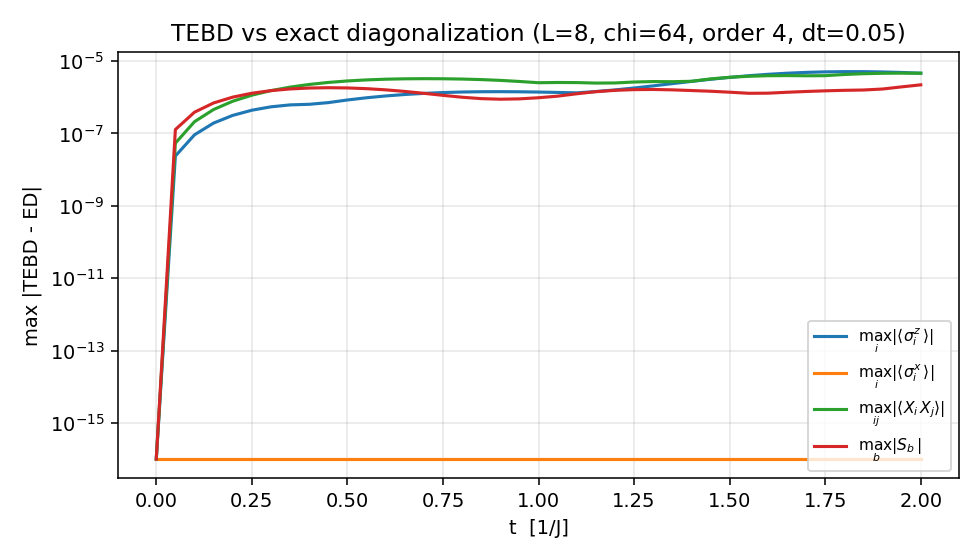
\includegraphics[width=0.75\textwidth]{figs/validate_errors.png}
\caption{Per-step max error of TEBD against exact diagonalisation. After the first step the error sits at the Trotter floor ($\sim 10^{-6}$) and stays there for the entire run; final state-vector fidelity loss is $4.3 \times 10^{-11}$.}
\end{figure}

\textbf{CPU runtime baseline (already collected).} $L = 20$, $dt = 0.05$, $t = 2$, order 4:

\begin{center}
\begin{tabular}{cc}
\toprule
$\chi_{\max}$ & wall (s) \\
\midrule
16  & 0.68 \\
32  & 2.99 \\
64  & 7.06 \\
128 & 7.13 \\
\bottomrule
\end{tabular}
\end{center}

The $16 \to 32 \to 64$ progression is consistent with the expected $\mathcal{O}(\chi^3)$ scaling. The plateau at $\chi_{\max} \ge 64$ requires a careful explanation: $\chi_{\max}$ is only an \emph{upper bound} on the bond dimension, not its actual value. The cost of each \texttt{update\_bond} is governed by the \emph{current} bond dimension $\chi_{\mathrm{actual}}(t)$, since the SVD operates on a $2\chi_{\mathrm{actual}} \times 2\chi_{\mathrm{actual}}$ matrix. From Fig.~1, $\chi_{\mathrm{actual}}(t)$ reaches the cap of 64 only at $t \approx 1.9$, so for the entire $t \in [0, 2]$ window the running SVDs are at most $128 \times 128$ --- and raising $\chi_{\max}$ to 128 cannot make those matrices any larger. The only effect of a larger $\chi_{\max}$ is more pre-allocated memory and fewer truncation events, neither of which adds compute. If we extended the run past $t \approx 2$, the $\chi_{\max} = 64$ curve would stay flat (capped) while the $\chi_{\max} = 128$ curve would keep growing as $\chi_{\mathrm{actual}}$ continued to climb --- and the runtime gap would open. Linear scaling in $L$ is observed at fixed $\chi_{\max}$.

\begin{figure}[h]
\centering
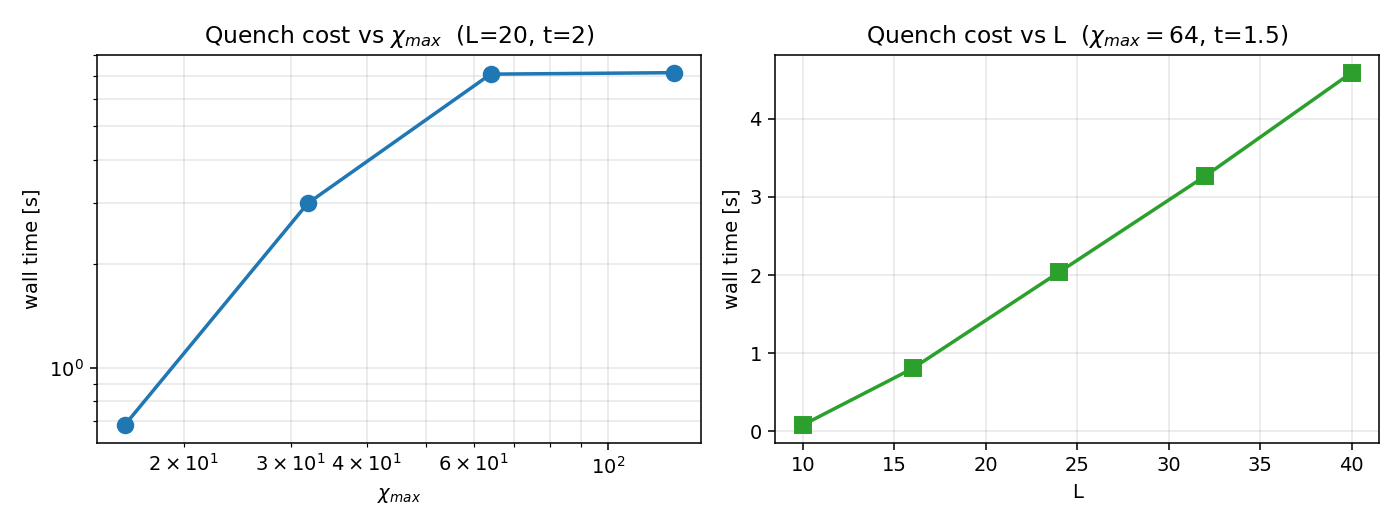
\includegraphics[width=\textwidth]{figs/bench.png}
\caption{Wall time vs $\chi_{\max}$ (left, log--log) and vs $L$ (right). Cubic scaling at small $\chi_{\max}$; flat once $\chi_{\mathrm{actual}}(t)$ is the binding dimension. Linear in $L$ at fixed $\chi_{\max}$.}
\end{figure}

\textbf{Experiments planned for M3 (CUDA):}
\begin{itemize}
    \item per-kernel timing breakdown via Nsight Systems (\texttt{gate\_apply}, \texttt{svd}, \texttt{vidal\_restore}, host$\leftrightarrow$device transfers);
    \item roofline of \texttt{update\_bond} via Nsight Compute, classifying each kernel as compute- or memory-bound;
    \item CPU vs.\ GPU speed-up curve over $\chi_{\max} \in \{16, 32, 64, 128, 256\}$;
    \item Jacobi-SVD sweep count vs.\ residual;
    \item peak device memory; verify zero \texttt{cudaMalloc} during evolution.
\end{itemize}

\textbf{Experiments planned for M4 (MPI):}
\begin{itemize}
    \item weak scaling on the embarrassingly-parallel parameter-sweep mode for $n_{\mathrm{GPU}} \in \{1, 2, 4, 8\}$;
    \item (stretch) strong scaling for spatial decomposition at $L = 64$.
\end{itemize}

What we hope to learn: (i) is single-chain TEBD compute-bound (SVD) or memory-bound (transposes) on a modern GPU? (ii) does Jacobi SVD remain practical at $\chi = 256$, or do we need a randomised SVD? (iii) is spatial MPI decomposition worth the complexity, or is sweep-parallelism the only useful mode?

\vspace{0.4em}
\textbf{7. Timeline}

\begin{itemize}
    \item \textbf{M3 --- GPU kernels (due May 11).} CUDA build setup; port \texttt{Tensor} / \texttt{TensorAccessor}, \texttt{zgemm}, \texttt{tensor\_contract}; port Jacobi \texttt{svd} and the fused \texttt{update\_bond} kernel; re-run all unit tests and \texttt{validate\_tebd\_vs\_ed} on the GPU path.

    \item \textbf{Profiling \& tuning.} Nsight timing breakdown, roofline analysis, optimise the dominant kernel, generate CPU-vs-GPU speed-up curves.

    \item \textbf{M4 --- Distributed (due May 27).} MPI parameter-sweep mode and weak-scaling numbers; if time allows, prototype spatial decomposition on $L = 64$.

    \item \textbf{Final report (due Jun 8).} Larger physics sweep across the TFIM phase diagram, write-up, buffer for debugging.
\end{itemize}

\textbf{Risks.} If Jacobi SVD underperforms cuSOLVER's batched SVD at large $\chi$, we keep the Jacobi kernel as the hand-written deliverable but switch the production path to \texttt{cusolverDnZgesvdjBatched}. If spatial MPI proves unproductive, parameter-sweep mode is the guaranteed fallback.

\end{document}
